\documentclass{beamer}
\usepackage{siunitx}
\usepackage{physics}

\usepackage[utf8]{inputenc}
\usetheme{Warsaw}
\title{Principal Component Analysis}
\author{JAYANT RANGI(MA17BTECH11006) \newline RITESH YADAV(MA17BTECH11009) }  


\begin{document}

\maketitle

\begin{frame}{Definition :}
\textbf{Orthogonal projection} of data onto lower-dimension linear space that...
\begin{itemize}
\newline
\item maximizes variance of projected data
\newline
\item minimizes mean squared distance between
\newline
\hspace{1cm}\begin{itemize}
    \item data points and
    \newline
    \item projections
\end{itemize}
\end{itemize}
\end{frame}
\begin{frame}{Random 2D Gaussian Data set :}
\centering
    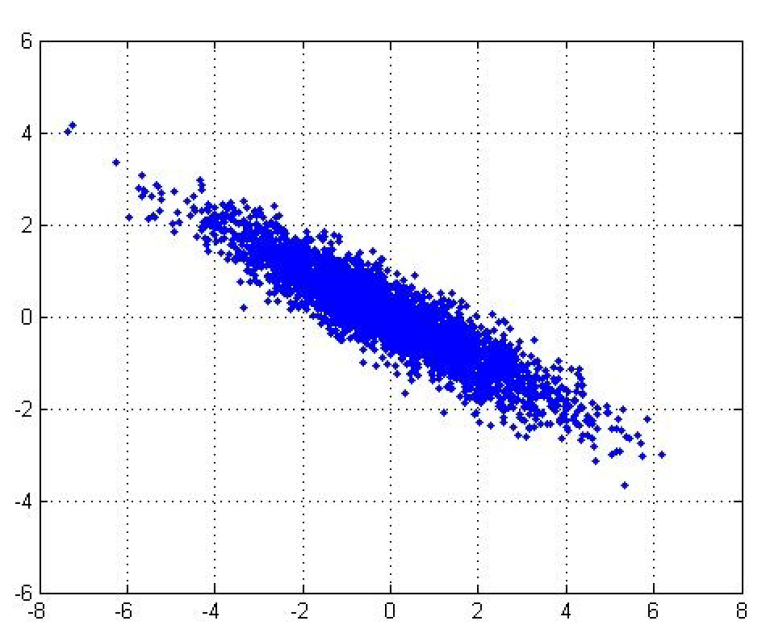
\includegraphics[scale=0.5]{2.png}
\end{frame}{}
\begin{frame}{1st PCA axis :}
\centering
    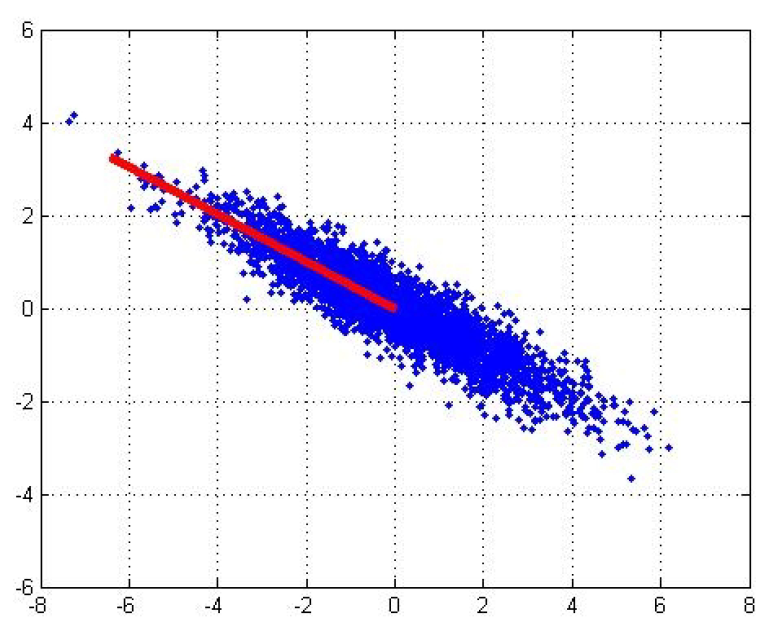
\includegraphics[scale=0.5]{3.png}
\end{frame}{}
\begin{frame}{2st PCA axis :}
\centering
    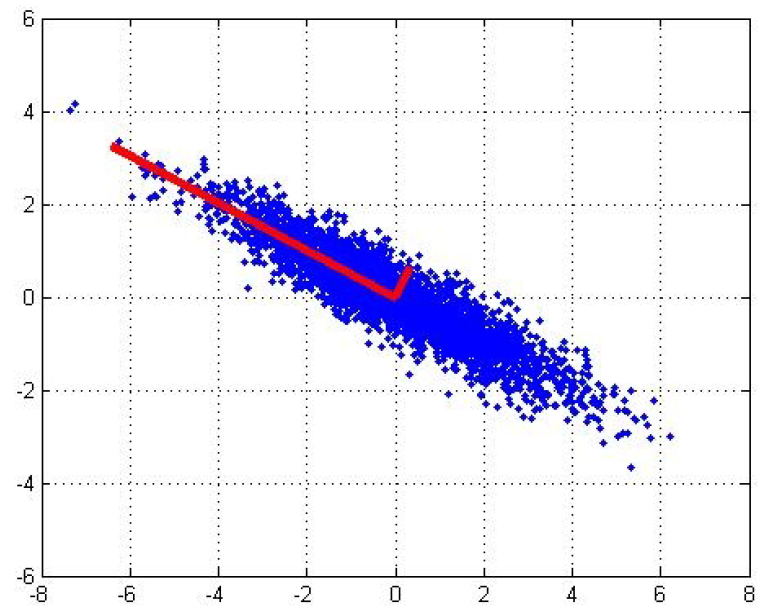
\includegraphics[scale=0.5]{4.png}
\end{frame}{}
\begin{frame}{Idea :}
\begin{itemize}
\item Given data points in a \textbf{d-dimensional} space,
project into \textbf{lower dimensional} space while
preserving as much information as possible
\newline
\newline
\item In particular, choose projection that
\textbf{minimizes squared error} in reconstructing original data
\end{itemize}    
\end{frame}

\begin{frame}{Applications :}
\begin{itemize}
\item \textbf{Data Visualization}
\newline
\item \textbf{Data Compression}
\newline
\item \textbf{Noise Reduction}
\newline
\item \textbf{Data Classification}
\newline
\item \textbf{Trend Analysis}
\newline
\item \textbf{Factor Analysis}
\end{itemize}
    
\end{frame}

\begin{frame}{Example :}
Let's take an example :
\newline
\begin{itemize}
\item You are given data of 53 different features from 65 people.
\newline
\item \textbf{How can you visualize such larger measurements?}
\newline
\newline
\end{itemize}
Now consider the given graph : 
\end{frame}
\begin{frame}{Spectral Format :}
\centering
    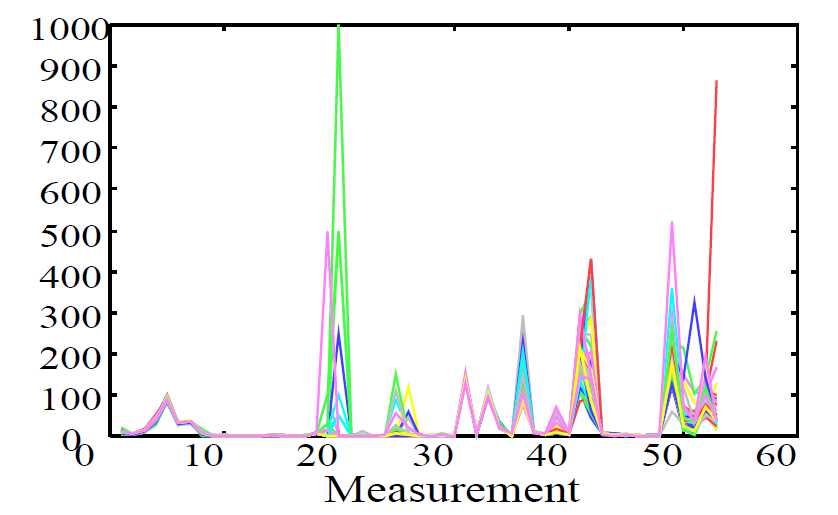
\includegraphics[scale=0.4]{1.png}
\newline    
\textbf{Difficult to compare different features by the above Graph .}    
\end{frame}{}
\begin{frame}{Conclusion From The Example :}
\begin{itemize}
\item Is there a representation better than the coordinate axes?
\newline
\item Is it really necessary to show all the 53 dimensions?
\textbf{what if there are strong correlations between the
features?}
\newline
\newline
\end{itemize}
\textbf{Principal Component Analysis} helps us in dealing such situations by removing the irrelevant information and keeping the strongly relevant information .
\end{frame}
\begin{frame}{Mathematics behind Principal Components Analysis:}
The principal components of a set of data in $|R^p$
provide a sequence of best
linear approximations to that data, of all ranks \newline q $\leq$ p
\newline
Denote the observations by $x_1,x_2,... ,x_N$ , and consider the rank-q linear
model for representing them. \newline
$f(\lambda) = \mu + \textbf{V}_q\lambda $ \newline
$\mu$ is a location vector in $R^p$.\newline
$V_q$ is a p\cross q matrix with q orthogonal
unit vectors as columns, and $\lambda$ is a q vector of parameters. This is the
parametric representation of an affine hyperplane of rank q.\newline
To fit this model to data we will use least squares approximation .

\end{frame}
\begin{frame}{Mathematics behind Principal Components Analysis:}
\underset{\mu,\lambda_i,\textbf{V}_q}{\text{min}} \sum_{n=1}^{N} ||x_i ${-}$ \mu ${-}$ \textbf{V}_q\lambda_i||^2 \newline \newline
\mu = \overline{x}
\newline
$\lambda_i=\textbf{V}_q^T(x_i-\overline{x})$ \newline
This leaves us to find the orthogonal matrix \textbf{V}_q : \newline \newline
$\underset{\textbf{V}_q}{\text{min}} \sum_{n=1}^{N} ||(x_i-\overline{x})-\textbf{V}_q\textbf{V}_q^T(x_i-\overline{x}) ||^2 $\newline \newline
For convenience we assume $\overline{x}=0 $\newline
The p\crossp matrix $\textbf{H}_q=\textbf{V}_q\textbf{V}_q^T$ is a a projection matrix, and maps each point $x_i$ onto its rank-q recontruction $\textbf{H}_qx_i$, the orthogonal projection of $x_i$ onto the subspace spanned by columns of $\textbf{V}_q$. 


\end{frame}
\end{document}
